\section{Subconjuntos}
\markright{SUBCONJUNTOS}

\subsection{Conjuntos y subconjuntos}

Un conjunto no es nada mas que una colección de objetos. Por ejemplo, si alguien trae en su mochila un plátano, manzana y naranja, este puede decir que trae un conjunto de frutas compuesto por un plátano, manzana y naranja.

En matemáticas e informática, nosotros estamos trabajando todo el rato con los conjuntos. Ya sean el conjunto de datos de entrada, o los números enteros, tener noción de conjuntos es un requerimiento para el éxito en la olimpiada.

Veamos un poco de notación. Para escribir el conjunto A de números esta conformado por el 3, 5 y 9 escribimos lo siguiente:
\[A=\{3,5,9\}\]

\begin{center}
	\textbf{TODO: CORREGIR ESTO}
\end{center}
\pagebreak

\subsection*{Ejemplo: Enlistar subconjuntos}
Veamos como hacer para visitar todos los subconjuntos, lo cuál será necesario para problemas donde nos preguntan por ellos.

Para esto, primero aprendamos a resolver el problema que trata de mostrar los subconjuntos:

\subsection*{Problema:}

Karel tiene un conjunto formado por las primeras \(N\) letras del alfabeto. Ahora Karel que imprimas todos los subconjuntos, uno por cada línea. Puedes imprimirlos en cualquier orden.

Cada subconjunto es representado por las letras en el de la A a la Z. El subconjunto vacío será representado por un asterisco '*'.

\textbf{Entrada}\\
Un entero \(N\), indicando cuantas letras hay en el conjunto.

\textbf{Salida}\\
Todos los subconjuntos

\textbf{Ejemplos}\\
\begin{casebox2}
	
	\scase{2}{
		AB\\
		A \\
		B\\
		*
	}
	\hline
\end{casebox2}

\begin{casebox2}
	\scase{3}
	{
		ABC \\
		AB \\
		AC\\
		A\\
		BC\\
		B\\
		C\\
		* \\
	}
	\hline
\end{casebox2}

\textbf{Límites}
\begin{plimits}
	\item \(1\leq N \leq 20 \)
\end{plimits}

\subsection*{Solución}

Entonces, podemos resolver el problema si obtenemos todos los subconjuntos posibles. Para esto, haremos un algoritmo que construya todos los posibles subconjuntos.

Esto se puede hacer de dos formas principales, una iterativa y otra recursiva. Comencemos viendo la forma con recursión.

\subsubsection* {Subconjuntos usando recursión}

Digamos que \(S(conjunto)\) sean todos los subconjuntos del \(conjunto\). Por ejemplo:
\[S(\{A,B,C\})=\]
\[\{\{A,B,C\},\{A,B\},	\{A,C\},\{A\},\{B,C\},	\{B\},\{C\},	\emptyset\} \]

O usando la misma notación que la salida del problema (la que usaremos a partir de aquí):

\[S(ABC)=\{ABC, AB, AC, A, BC, B, C, * \}\]

Veamos un poco como se comporta S, por ejemplo para \(N = 4\), en total tenemos 16 subconjuntos los cuales podemos dividir en dos mitades con 8 cada una, los que tienen la A y los que no tienen la A.



\begin{center}
	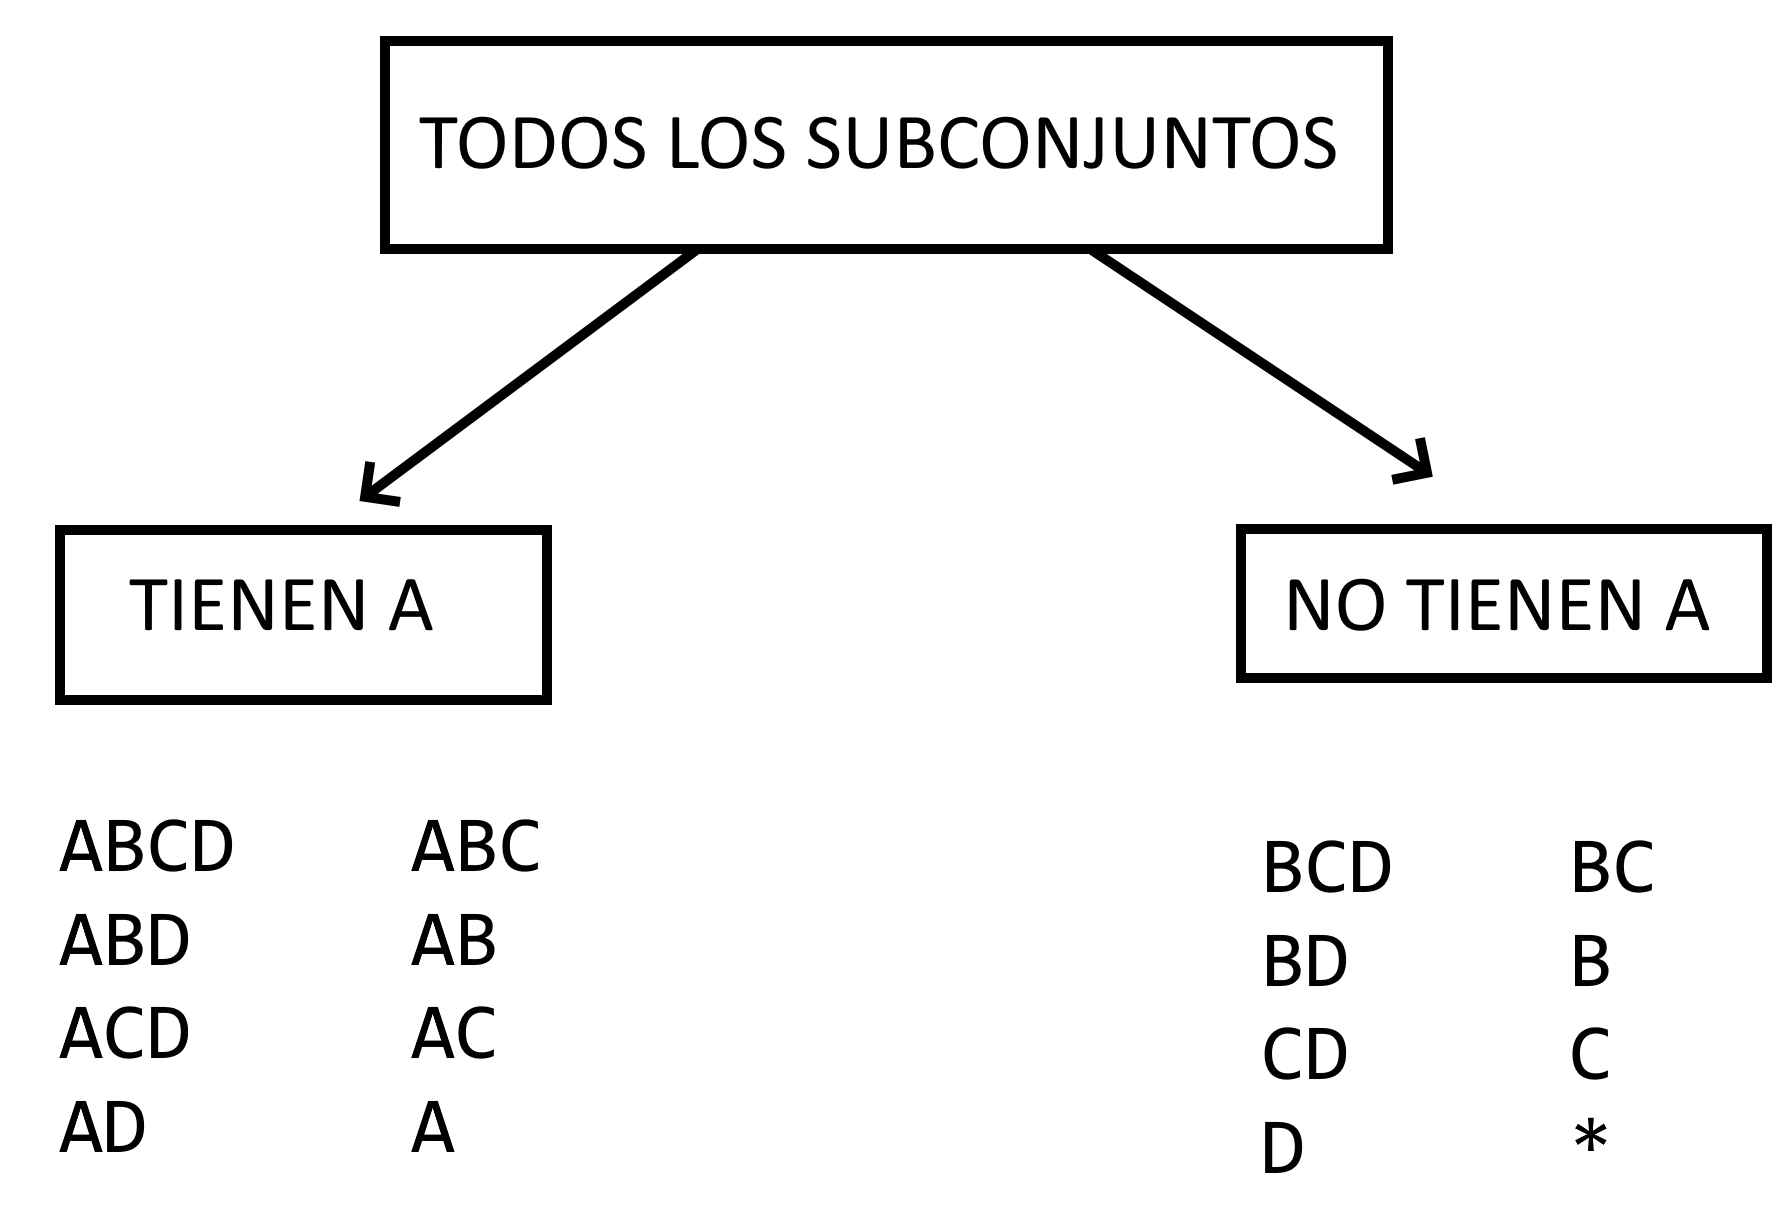
\includegraphics[scale=0.15]{subconjuntos1}
\end{center}

Ahora veamos que para los dos grupos, tenemos todos los 8 subconjuntos para \(BCD\), y lo único que los diferencia es si tienen \(A\) al inicio o no. Si supiéramos cuales son esos subconjuntos para las ultimas 3 letras, podríamos perfectamente construir \(S(ABCD)\), 

En concreto, podemos ver que \(S(ABCD) \) es igual a \(S(BCD)\) con \(A\) al inicio y \(S(BCD)\) sin nada extra. 

Si lo quieres ver en formula sería similar a \(S(ABCD)=A\rightarrow S(BCD) \cup S(BCD)\), donde \(A\rightarrow S(BCD)\) significa agregar \(A\) a todos los subconjuntos en \(S(BCD)\).

Y podemos hacer lo mismo, ver que \(S(BCD)\) es otra vez: los subconjuntos de \(CD\) con B y sin B.

Y de aquí obtenemos nuestro comportamiento recursivo.

Ahora que vemos la recursión, veamos una forma de implementar todo esto para resolver el problema.

Crearemos un metodo construyeSubconjuntos(int pos, int previo) que constuya los subconjuntos usando las letras desde pos hasta \(N-1\).
\pagebreak
\begin{lstlisting}
	#include <iostream>
	using namespace std;
	int N;
	char subconjunto[25];
	
	// pos implica que letra estamos eligiendo si esta o no A=0, B=1, C=2, ...
	// para N=6, pos = 2, es equivalente a  S(CDEF)
	// previo indica cuantas letras se han agregaron a la construccion.
	void construyeSubconjuntos(int pos, int previo) {
		if (pos == N) {
			//Ya no hay mas letras que decidir
			//imprime el subconjunto construido.
			if (previo==0) {
				cout <<"*\n";
			} else {
				cout << subconjunto<<"\n"; 
			}
			return;
		}
		//agrega la letra pos a la construccion
		subconjunto[previo]=pos+'A'; 
		construyeSubconjuntos(pos+1, previo+1); 
		
		// Quita la letra pos de la construccion
		subconjunto[previo]='\0'; 
		construyeSubconjuntos(pos+1, previo); 
		
	}
	
	int main () {
		cin >> N;
		construyeSubconjuntos(0,0);
		return 0;
	}
\end{lstlisting}


De forma que el árbol de la recursión para construyeSubconjuntos(0,0) con \(N=2\) se ve:

\begin{center}
	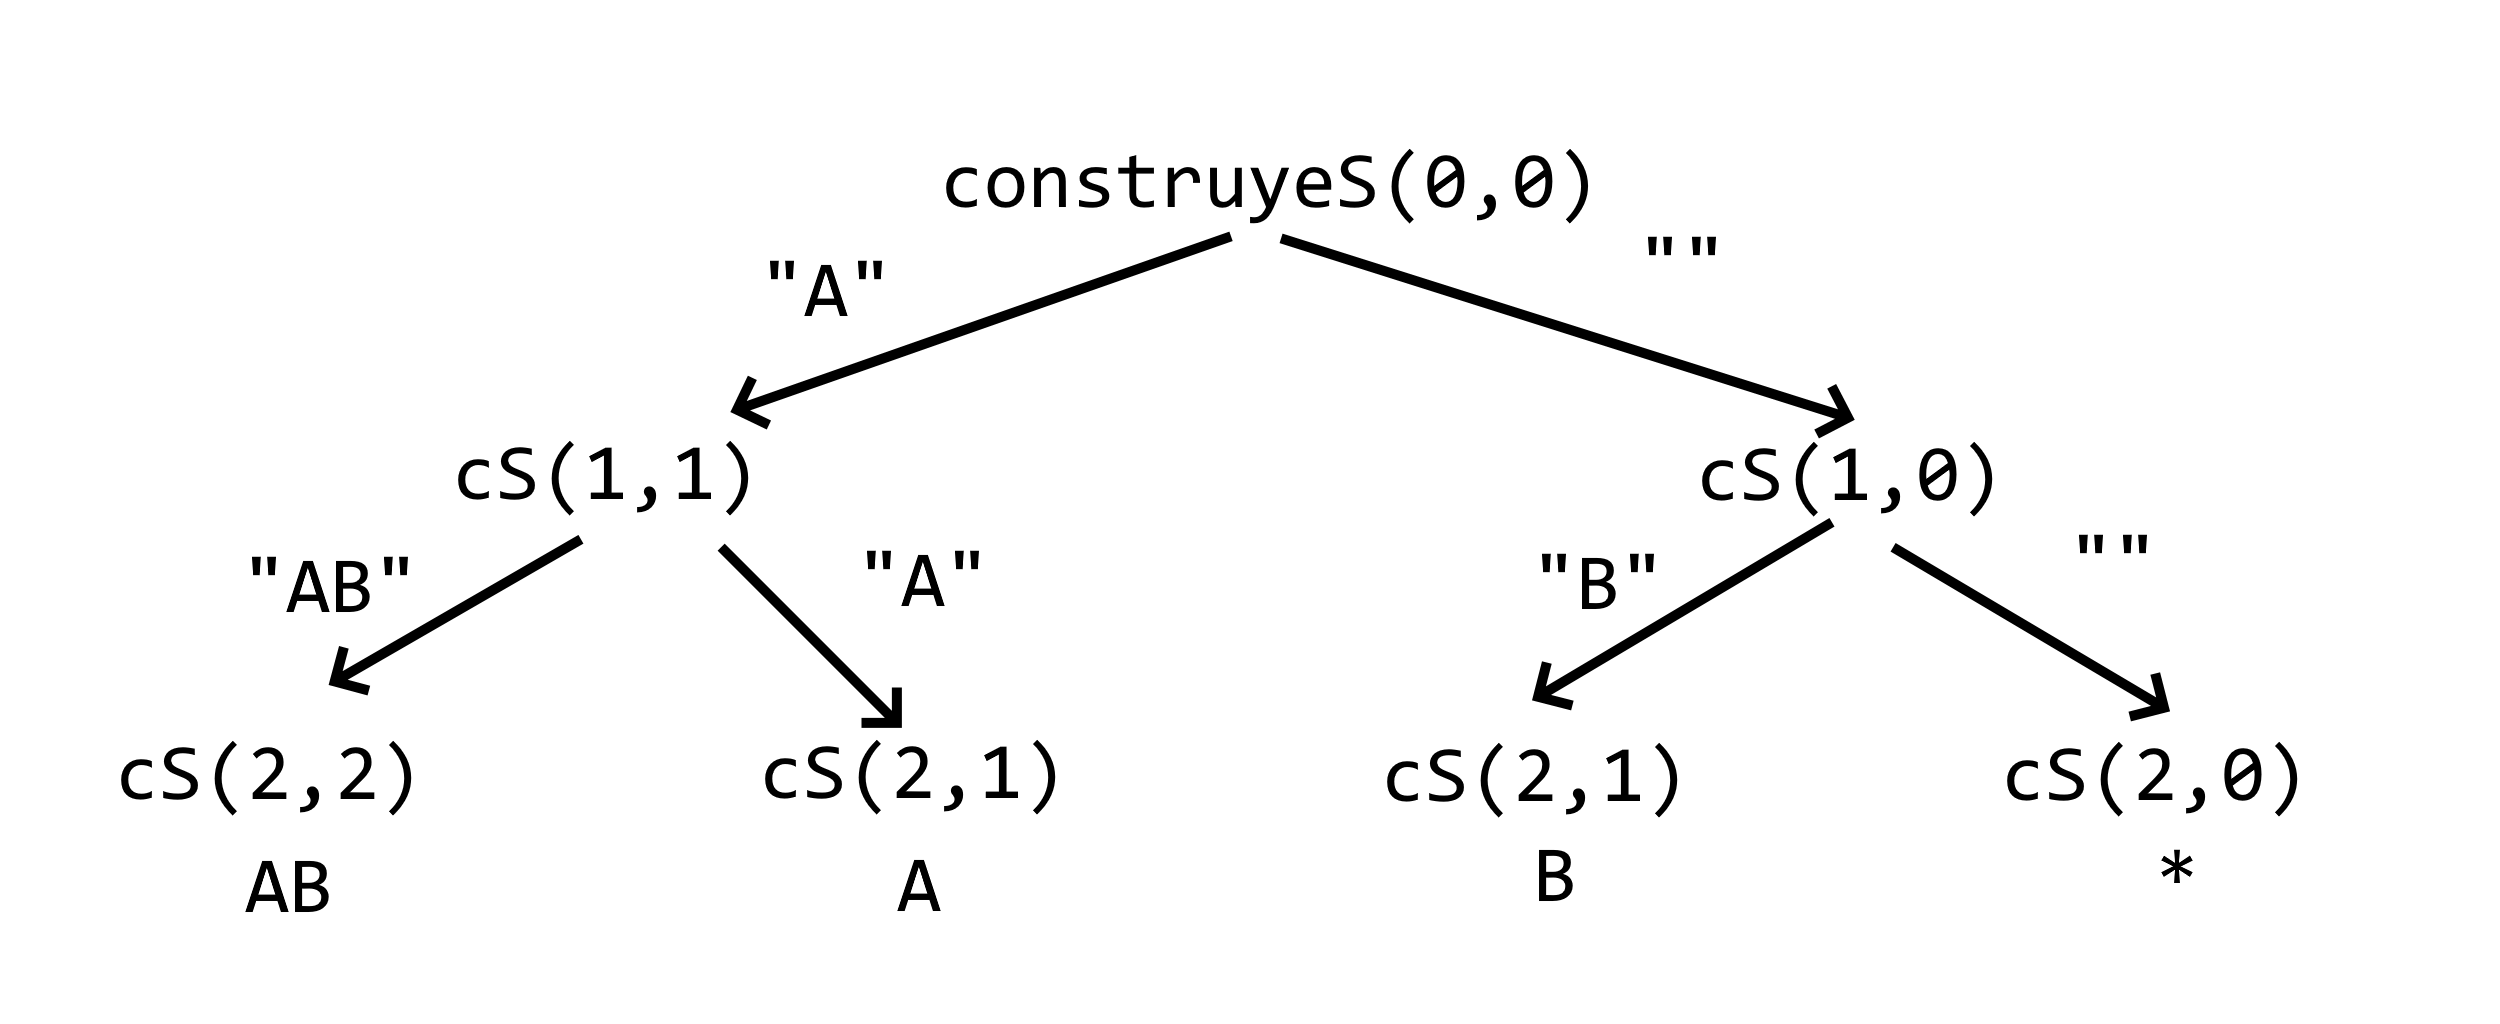
\includegraphics[scale=0.15]{AB}
\end{center} 

\subsection{Complejidad}

a complejidad de este código es igual a la cantidad de subconjuntos que se tienen con \(N\) elementos.

La primera forma de hacerlo es darnos cuenta que cada elemento tiene dos opciones, estar o no estar, por principio multiplicativo vemos que se multiplica por dos tantas veces como elementos tengamos. En total es \(2^N\) 

Esto es observable si recordamos el diagrama de las llamadas recursivas.

Vemos que por cada elemento, se divide en dos, duplicando la cantidad de llamadas en el proceso. En el primer nivel con pos=0, tenemos solo una llamada, con pos=1 tenemos dos, pos=3 obtenemos cuatro y así sucesivamente.

Por lo tanto, la complejidad es \(O(2^N)\), exponencial.

Una vez comprendido esto, pasemos a utilizar esto para resolver problemas.

\subsection*{Ejemplo Subconjunto de Suma K}
Fernando ha llegado a la ferretería con su objetivo frecuente de comprar \(K\) tornillos.  Sin embargo, la ferretería no siempre vende cajas con exactamente \(K\) tornillos dentro.

La ferretería tiene \(N\) cajas diferentes en venta, cada uno con \(C_i\) tornillos dentro.

Fernando quiere comprar unas cuantas cajas y obtener \textbf{exactamente} \(K\) tornillos. Por fortuna, esta vez trajo una bolsa y podrá comprar cuantas cajas le sea necesario.

Conociendo las cajas que venden en la Ferretería, determina si Fernando puede comprar los \(K\).

\textbf{Entrada}\\
Dos enteros \(N\) y \(K\), la cantidad de cajas en la Ferretería y cuantos tornillos quiere Fernando.

En la siguiente línea vendrán la cantidad de tornillos en cada caja, los valores \(C_i\), separados por espacios.

\textbf{Salida}\\
Debes imprimir "SI" en caso de que Fernando pueda comprar exactamente \(K\) tornillos. Caso contrario, imprime "NO".

\textbf{Ejemplos}\\
\begin{casebox3}
	\ecase{
		5 10\\
		2 4 5 3 9	
	}
	{SI}
	{
		Compra la primera, tercera\\
		y cuarta caja.
	}
	\ecase{
		5 12\\
		4 5 2 11 3	
	}
	{NO}
	{}
\end{casebox3}

\textbf{Límites}
\begin{plimits}
	\item \(1\leq N\leq 20 \)
	\item \(1\leq C_i\leq 10^9 \)
	\item \(1\leq K\leq 10^9 \)
\end{plimits}

\subsection*{Solución}
Como siempre, resumamos el problema en menos palabras. En corto, nos preguntan si existe un subconjunto de cajas tal que la suma de sus valores sea exactamente \(K\).

Y como es propio de todos los subtemas de búsqueda completa, veamos todas las posibles soluciones, es decir todos los subconjuntos, hasta que encontremos el que cumpla la condición o nos quedemos sin opciones.

Como ya vimos la forma de iterar por todos los subconjuntos en el ejemplo 3.1, utilicemos esas ideas para resolver este problema.

Lo que podemos hacer es ir construyendo todos los subconjuntos, esta vez en vez de representarlos como una cadena, lo representaremos como su suma. Esto en código se ve:
\newpage
\begin{lstlisting}
	int Cajas[25];
	int N;
	long long K;
	// Aqui, llevamos la suma del subconjunto construido
	void buscaSubconjunto(int pos, long long suma) {
		if (pos==N) {
			if (suma == K) {
				/* Encontramos un subconjunto con suma K.
				Imprimmos SI y terminemos el programa */
				cout << "SI";
				exit(0);
			}
			return;
		}
		buscaSubconjunto(pos+1, suma+Cajas[pos]);//Incluyamos pos en el subconjunto
		buscaSubconjunto(pos+1, suma);//Excluyamos pos del subconjunto	
	}
	
	int main () {
		ios_base::sync_with_stdio(0); cin.tie(0);
		cin >> N >>K;
		for (int i=0; i < N; i++) {
			cin >> Cajas[i];
		}
		buscaSubconjunto(0,0);
		//Si llegamos aqui es porque nunca encontramos la respuesta.
		cout << "NO";
		return 0;
	}
\end{lstlisting}

